\documentclass[11pt]{article}
\usepackage{../pplmanual}
\NeedsTeXFormat{LaTeX2e}
\typeout{^^J^^J
Parallel Programming Laboratory^^J
Manual Style^^J
Written by Milind A. Bhandarkar, 12/00^^J}

%%% Make it possible for both ps and pdf to be generated
\newif\ifpdf
\ifx\pdfoutput\undefined
  \pdffalse
\else
  \pdfoutput=1
  \pdftrue
\fi

\ifpdf
  \pdfcompresslevel=9
\fi

%%% Imported from fullpage.sty, since it is not always available
\topmargin 0pt
\advance \topmargin by -\headheight
\advance \topmargin by -\headsep

\textheight 8.9in

\oddsidemargin 0pt
\evensidemargin \oddsidemargin
\marginparwidth 1.0in

\textwidth 6.5in
%%% end import from fullpage

%%% Commonly Needed packages
\usepackage{graphicx,color,calc}
\usepackage{makeidx}
\usepackage{alltt}

%%% Commands for uniform looks of C++, Charm++, and Projections
\newcommand{\CC}{C\kern -0.0em\raise 0.5ex\hbox{\normalsize++}}
\newcommand{\emCC}{C\kern -0.0em\raise 0.4ex\hbox{\normalsize\em++}}
\newcommand{\charmpp}{\sc Charm++}
\newcommand{\projections}{\sc Projections}
\newcommand{\converse}{\sc Converse}
\newcommand{\ampi}{\sc AMPI}

%%% Commands to produce margin symbols
\newcommand{\new}{\marginpar{\fbox{\bf$\mathcal{NEW}$}}}
\newcommand{\important}{\marginpar{\fbox{\bf\Huge !}}}
\newcommand{\experimental}{\marginpar{\fbox{\bf\Huge $\beta$}}}

%%% Commands for manual elements
\newcommand{\zap}[1]{ }
\newcommand{\function}[1]{{\noindent{\textsf{#1}}\\}}
\newcommand{\cmd}[1]{{\noindent{\textsf{#1}}\\}}
\newcommand{\args}[1]{\hspace*{2em}{\texttt{#1}}\\}
\newcommand{\param}[1]{{\texttt{#1}}}
\newcommand{\kw}[1]{{\textsf{#1}}}
\newcommand{\uw}[1]{{\textsl{#1}}}
\newcommand{\desc}[1]{\indent{#1}}

%%% Commands needed for Maketitle
\newcommand{\@version}{}
\newcommand{\@credits}{}
\newcommand{\version}[1]{\renewcommand{\@version}{#1}}
\newcommand{\credits}[1]{\renewcommand{\@credits}{#1}}

%%% Print the License Page
\newcommand{\@license}{%
 \begin{center}
   {University of Illinois}\\
   {\charmpp/\converse\ Parallel Programming System Software}\\
   {Non-Exclusive, Non-Commercial Use License}\\
 \end{center}
 \rule{\textwidth}{1pt}
{\tiny
Upon execution of this Agreement by the party identified below (``Licensee''),
The Board of Trustees of the University of Illinois  (``Illinois''), on behalf
of The Parallel Programming Laboratory (``PPL'') in the Department of Computer
Science, will provide the \charmpp/\converse\ Parallel Programming System
software (``\charmpp'') in Binary Code and/or Source Code form (``Software'')
to Licensee, subject to the following terms and conditions. For purposes of
this Agreement, Binary Code is the compiled code, which is ready to run on
Licensee's computer.  Source code consists of a set of files which contain the
actual program commands that are compiled to form the Binary Code.

\begin{enumerate}
  \item
    The Software is intellectual property owned by Illinois, and all right,
title and interest, including copyright, remain with Illinois.  Illinois
grants, and Licensee hereby accepts, a restricted, non-exclusive,
non-transferable license to use the Software for academic, research and
internal business purposes only, e.g. not for commercial use (see Clause 7
below), without a fee.

  \item 
    Licensee may, at its own expense, create and freely distribute
complimentary works that interoperate with the Software, directing others to
the PPL server (\texttt{http://charm.cs.uiuc.edu}) to license and obtain the
Software itself. Licensee may, at its own expense, modify the Software to make
derivative works.  Except as explicitly provided below, this License shall
apply to any derivative work as it does to the original Software distributed by
Illinois.  Any derivative work should be clearly marked and renamed to notify
users that it is a modified version and not the original Software distributed
by Illinois.  Licensee agrees to reproduce the copyright notice and other
proprietary markings on any derivative work and to include in the documentation
of such work the acknowledgement:

\begin{quote}
``This software includes code developed by the Parallel Programming Laboratory
in the Department of Computer Science at the University of Illinois at
Urbana-Champaign.''
\end{quote}

Licensee may redistribute without restriction works with up to 1/2 of their
non-comment source code derived from at most 1/10 of the non-comment source
code developed by Illinois and contained in the Software, provided that the
above directions for notice and acknowledgement are observed.  Any other
distribution of the Software or any derivative work requires a separate license
with Illinois.  Licensee may contact Illinois (\texttt{kale@cs.uiuc.edu}) to
negotiate an appropriate license for such distribution.

  \item
    Except as expressly set forth in this Agreement, THIS SOFTWARE IS PROVIDED
``AS IS'' AND ILLINOIS MAKES NO REPRESENTATIONS AND EXTENDS NO WARRANTIES OF
ANY KIND, EITHER EXPRESS OR IMPLIED, INCLUDING BUT NOT LIMITED TO WARRANTIES OR
MERCHANTABILITY OR FITNESS FOR A PARTICULAR PURPOSE, OR THAT THE USE OF THE
SOFTWARE WILL NOT INFRINGE ANY PATENT, TRADEMARK, OR OTHER RIGHTS.  LICENSEE
ASSUMES THE ENTIRE RISK AS TO THE RESULTS AND PERFORMANCE OF THE SOFTWARE
AND/OR ASSOCIATED MATERIALS.  LICENSEE AGREES THAT UNIVERSITY SHALL NOT BE HELD
LIABLE FOR ANY DIRECT, INDIRECT, CONSEQUENTIAL, OR INCIDENTAL DAMAGES WITH
RESPECT TO ANY CLAIM BY LICENSEE OR ANY THIRD PARTY ON ACCOUNT OF OR ARISING
FROM THIS AGREEMENT OR USE OF THE SOFTWARE AND/OR ASSOCIATED MATERIALS.

  \item 
    Licensee understands the Software is proprietary to Illinois. Licensee
agrees to take all reasonable steps to insure that the Software is  protected
and secured from unauthorized disclosure, use, or release and  will treat it
with at least the same level of care as Licensee would use to  protect and
secure its own proprietary computer programs and/or information, but using no
less than a reasonable standard of care.  Licensee agrees to provide the
Software only to any other person or entity who has registered with Illinois.
If licensee is not registering as an individual but as an institution or
corporation each member of the institution or corporation who has access to or
uses Software must agree to and abide by the terms of this license. If Licensee
becomes aware of any unauthorized licensing, copying or use of the Software,
Licensee shall promptly notify Illinois in writing. Licensee expressly agrees
to use the Software only in the manner and for the specific uses authorized in
this Agreement.

  \item
    By using or copying this Software, Licensee agrees to abide by the
copyright law and all other applicable laws of the U.S. including, but not
limited to, export control laws and the terms of this license. Illinois  shall
have the right to terminate this license immediately by written  notice upon
Licensee's breach of, or non-compliance with, any terms of the license.
Licensee may be held legally responsible for any  copyright infringement that
is caused or encouraged by its failure to  abide by the terms of this license.
Upon termination, Licensee agrees to  destroy all copies of the Software in its
possession and to verify such  destruction in writing.

  \item
  The user agrees that any reports or published results obtained with  the
Software will acknowledge its use by the appropriate citation as  follows:

\begin{quote}
``\charmpp/\converse\ was developed by the Parallel Programming Laboratory in
the Department of Computer Science at the University of  Illinois at
Urbana-Champaign.''
\end{quote}

Any published work which utilizes \charmpp\ shall include the following
reference:

\begin{quote}
``L. V. Kale and S. Krishnan. \charmpp: Parallel Programming with Message-Driven
Objects. In 'Parallel Programming using \CC' (Eds. Gregory V. Wilson and Paul
Lu), pp 175-213, MIT Press, 1996.''
\end{quote}

Any published work which utilizes \converse\ shall include the following
reference:

\begin{quote}
``L. V. Kale, Milind Bhandarkar, Narain Jagathesan, Sanjeev Krishnan and Joshua
Yelon. \converse: An Interoperable Framework for Parallel Programming.
Proceedings of the 10th International Parallel Processing Symposium, pp
212-217, April 1996.''
\end{quote}

Electronic documents will include a direct link to the official \charmpp\ page
at \texttt{http://charm.cs.uiuc.edu/}

  \item
    Commercial use of the Software, or derivative works based thereon,
REQUIRES A COMMERCIAL LICENSE.  Should Licensee wish to make commercial use of
the Software, Licensee will contact Illinois (kale@cs.uiuc.edu) to negotiate an
appropriate license for such use. Commercial use includes: 

    \begin{enumerate}
      \item
	integration of all or part of the Software into a product for sale,
lease or license by or on behalf of Licensee to third parties, or 

      \item
	distribution of the Software to third parties that need it to
commercialize product sold or licensed by or on behalf of Licensee.
    \end{enumerate}

  \item
    Government Rights. Because substantial governmental funds have been  used
in the development of \charmpp/\converse, any possession, use or sublicense of
the Software by or to the United States government shall be subject to such
required restrictions.

  \item
    \charmpp/\converse\ is being distributed as a research and teaching tool
and as such, PPL encourages contributions from users of the code that might, at
Illinois' sole discretion, be used or incorporated to make the basic  operating
framework of the Software a more stable, flexible, and/or useful  product.
Licensees who contribute their code to become an internal  portion of the
Software agree that such code may be distributed by  Illinois under the terms
of this License and may be required to sign an  ``Agreement Regarding
Contributory Code for \charmpp/\converse\ Software'' before Illinois  can
accept it (contact \texttt{kale@cs.uiuc.edu} for a copy).
\end{enumerate}

UNDERSTOOD AND AGREED.

Contact Information:

The best contact path for licensing issues is by e-mail to
\texttt{kale@cs.uiuc.edu} or send correspondence to:

\begin{quote}
Prof. L. V. Kale\\
Dept. of Computer Science\\
University of Illinois\\
1304 W. Springfield Ave\\
Urbana, Illinois 61801 USA\\
FAX: (217) 333-3501
\end{quote}
}%tiny
 \newpage
}% end of license

\renewcommand{\maketitle}{\begin{titlepage}%
 \begin{flushright}
   {\Large
     Parallel Programming Laboratory\\
     University of Illinois at Urbana-Champaign\\
   }
 \end{flushright}
 \rule{\textwidth}{3pt}
 \vspace{\fill}
 \begin{flushright}
   \textsf{\Huge \@title \\}
 \end{flushright}
 \vspace{\fill}
 \@credits \\
 \rule{\textwidth}{3pt}
 \begin{flushright}
   {\large Version \@version}
 \end{flushright}
 \end{titlepage}
 \@license

 \tableofcontents
 \newpage
}% maketitle



\makeindex

\title{Charj Manual \\ Compiler Support for Productive Parallel Programming \footnote{last modified 12/14/2012 by Bilge Acun}}
\version{1.0}
\begin{document}

\maketitle

\section{Introduction}

Charj is a new programming language which incorporates syntax, semantic analysis, and optimization targeted at HPC code with its associated compiler. 

\begin{figure}[h]
\begin{center}
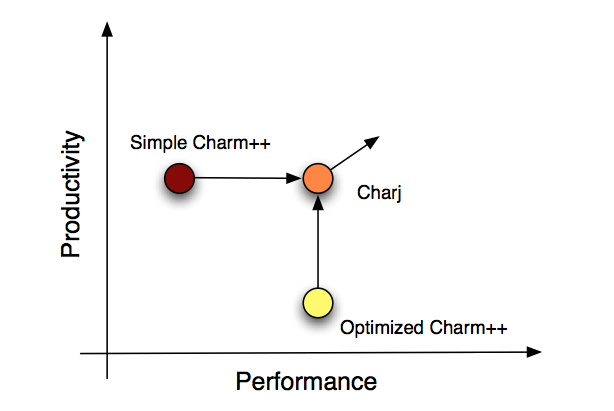
\includegraphics[width=4in]{fig/fig0.png}
\end{center}
\caption{Charj}
\label{fig:fig0}
\end{figure}

With Charj, we aim to allow programmers to achieve the performance associated with carefully written, hand-optimized Charm++ applications, but with much less time and effort. If effect, we hope to combine the productivity that programmers experience when writing relatively simple, naive applications while enjoying performance that would normally require a much greater investment of time, effort, and expertise. 

Charj compiler takes Charj codes as input and produces Charm++ interface (.ci) and C++ code (.C and .h) as an output. 

\begin{figure}[h]
\begin{center}
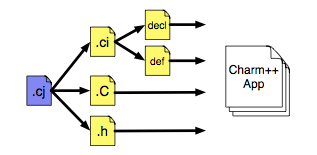
\includegraphics[width=4in]{fig/fig1.png}
\end{center}
\caption{Compilation process for Charj application}
\label{fig:fig1}
\end{figure}

\begin{verbatim}


\end{verbatim}

To make use of Charj;
\begin{enumerate}
\item Build Charm++, then build Charj
\item Write your Charj program
\item Compile and run it!
\end{enumerate}

\section{Building, Compiling and Running}
{\bf To write a program and compile with Charj:}

\begin{enumerate}
\item Go to: {\it charm/src/langs/charj} and {\it "make" } (Assuming Charm++ is already installed)
\item Write your Charj code in a file with {\it .cj} extension. {\it (SampleProgram.cj)}
\item Execute {\it charjc} script on the file {\it SampleProgram.cj}: \\ {\it charm/src/langs/charj/bin/charjc  SampleProgram.cj}
\item After execution, a folder named {\it“SampleProgram.cj.gen”} will be created in the directory of {\it SampleProgram.cj}. This folder will contain the emitted Charm++ files; {\it SampleProgram.ci, SampleProgram.h SampleProgram.cc }.

* Example Charj programs can be found at {\it charm/src/langs/charj/tests}
\end{enumerate}


\section{Writing a Charj Program}

\subsection{General structure of a Charj program; }

\begin{verbatim}

	readonly Main@ mainProxy;	//readonly proxy type
	readonly int value;			//readonly variable
	
	public mainchare Main {
	    public entry Main(CkArgMsg[~]@ m){...} 	//Main constructor
	    public entry void done(){...}		    	//entry method 
	    private int localMethod(int value){...} 	//non-entry method
	}
	public chare_array [1d] SampleChareArray1d{...}	//1d chare array
	public chare_array [2d] SampleChareArray2d{...}	//2d chare array

	public class SampleObject{...}					//sample class

	public chare SampleChare {
	    public entry SampleChare(){...}				//constructor
	    public entry SampleChare(boolean flag){...}	//constructor 2
	    public entry void test(SampleObject obj){...}	//entry method
	}

\end{verbatim}

\subsection{Chare creation and method calls: }

\begin{verbatim}
	SampleChare@ sp = new SampleChare@();
	SampleChareArray1d@ sp1 = new SampleChareArray1d@(x_dim);
	SampleChareArray2d@ sp2 = new SampleChareArray2d@(x_dim, y_dim);
	sp@test();
	sp1@test();
	sp1[index]@test();
	sp2@test(int value);
\end{verbatim}

\subsection{Arrays:}

\begin{verbatim}
	Array<int> foo = new Array<int>([10]);  //1d array of integers of size 10
	foo[i] = ...;
	Array<double, 2> foo2 = new Array<double, 2>([s1, s2]); //2d array of size s1, s2
	foo2[i, j] = ...;
\end{verbatim}

\subsection{SDAG statements:}
These statements can be used inside of any entry method.

\begin{verbatim}
	when receiveMsg(SampleObject obj) {...}

	overlap{	//two overlapping when statements
		when receiveMsg1[i](int iter, SampleObject obj) {...}
		when receiveMsg2[i](int iter, int value) {...}
	}
\end{verbatim}

\subsection{Extern statements: }
If you want to use any other C++ function/feature, you have to define it as {\it extern}.

\begin{verbatim}
	extern atoi;			//define in the beginning of the file
	int x = atoi(y);		//use anywhere
\end{verbatim}

\subsection{Reduction statements:}
Currently only plain reductions are supported.

\begin{verbatim}
	contribute(CkCallback(CkReductionTarget(Main, done), mainProxy));
\end{verbatim}

\subsection{Some Charm++ statements that can be used in a Charj program:}

\begin{verbatim}
	CkExit();
	CkPrintf();
	CkMyPe();
	CkNumPes();
	CkMyNode();
	CkNumNodes();
	CkWallTimer();
	thisProxy
	thisIndex
\end{verbatim}

\end{document}
